\paragraph{\trBasicMorphism。}\label{sub:basic-morphism}
设 $M$ 是一个\trExactSymplectic\trCorneredBoundary\trManifold，而 $V$ 是其中一张带\trFrame{}的\trExact\trLagrange\trSphere。利用\cref{thm:cochain-level-vanishing}的上链层面消没结果会对我们很方便，因此我们假设 $2c_1(M,V)$ 为零。令 $L_0=V$，并另取两个\trExact\trLagrange\trSubmanifold{}$L_1$、$L_2$，其性质为 $L_2$ \trIsotopy{}于 $\tau_V(L_1)$；更确切地说，我们要指定\trIsotopy{}的一个选取。我们还要为三对 $(L_0,L_1)$、$(L_0,L_2)$ 与 $(L_1,L_2)$ 取定\trFloerDatum，并为定义乘积 $\mu^2\colon CF^{\mathrm{pr}}(L_1,L_2)\otimes CF^{\mathrm{pr}}(L_0,L_1)\to CF^{\mathrm{pr}}(L_0,L_2)$ 所需的\trPerturbationDatum{}取定一个选取。为了与代数理论更好对照，我们把由 $L_0$、$L_1$、$L_2$ 给出的 $\scr{F}^{\mathrm{pr}}(M)$ 的那些\trObject{}记作 $Y_0$、$Y_1$、$Y_2$。
取定一个\trLefschetzFibration{}$\pi\colon E\to S$，它在一个\trDisk{}之上、以 $M$ 为\trFiber，具有唯一的\trCriticalPoint，其\trVanishingCycle{}为 $V$。更确切地说，我们要求这个\trFibration{}配有\trMarkedPoint{}$\ast\in\partial S$，以及在该点处把\trFiber{}$E_\ast$ 等同到 $M$ 的一个等同；它还应带有从 $\ast$ 出发的一条\trVanishingPath{}$\gamma$，使得 $V_\gamma=V$。出于技术简单性的考虑，我们进一步假定该\trFibration{}在 $\ast$ 附近局部平凡。在接下来的全部构造中，$E$ 都将是必不可少的基本构件；这些构造基本上都是在 $E$ 上\trGluing{}各种平凡的部件。
\begin{remark}\label{thm:fibrations-exist-by-hand}
回顾：这样的\trFibration{}对任何给定的 $M$ 与 $V$ 都存在，而且事实上可以“凭手工”构造出来（概述见\cref{sub:constructing-lefschetz-fibrations}，完整的论述见 [131, Lemma 1.10]）。若在构造的细节上多加留意，便能得到稍多的控制：该\trSymplectic\trConnection{}在\trCriticalPoint{}的一个小邻域之外将是\trFlat{}的；任何\trVanishingPath{}的\trVanishingCycle{}都等于 $V$；并且绕\trCriticalValue{}一周的任何\trLoop{}的\trMonodromy{}是一个 \trDehnTwist{}$\tau_V$（而不只是与之\trIsotopy）。然而，这些性质没有一条对我们的构造是必不可少的。
\end{remark}
作为第一个、也是最初等的应用，我们将定义一个\trFloer{}\trCocycle
\begin{equation}\label{eq:floer-cocycle-c}
\boxed{\begin{gathered}
c\in CF^{\mathrm{pr}}(L_1,L_2),\\
\mu^1(c)=0.
\end{gathered}}
\end{equation}
为此，我们取给定的 $E\to S$ 并把 $\ast$ 去掉。所得是一个\trLefschetzFibration{}$E^c\to S^c$，带有一个无穷远点，我们把它看作一个\trIncomingPoint。把这个点记作 $\zeta^{c,-}$，并选取一个\trStriplikeEnd{}$\epsilon_{\zeta^{c,-}}$。存在一个\trCanonical{}的（在相差逐\trFiber\trIsotopy{}的意义下）移动\trLagrange\trBoundaryCondition{}$F^c$，其定义如下。从 $\epsilon_{\zeta^{c,-}}(s,0)$（$s\ll0$）之上的各\trFiber{}中的 $L_1$ 出发；然后用\trParallelTransport{}带着它绕 $\partial S^c$ 行进几乎一整圈。所得结果\trIsotopy{}于 $\tau_V(L_1)$，因而也\trIsotopy{}于 $L_2$；我们用这个\trIsotopy{}把它连续地延拓，使其在 $\epsilon_{\zeta^{c,-}}(s,1)$（$s\ll0$）之上的各\trFiber{}中变得等于 $L_2$。
这一构造示意性地显示于\cref{fig:monodromy-cut-open}。在那里，图示记法是：先把诸\trSingularFibre{}去掉，再沿虚线把基剪开，得到一个平凡的\trSymplectic\trFibration。此时的\trMonodromy{}就被看作是切口两侧之间的一个等同。在这类图中，我们通常不区分相互\trIsotopy{}的\trObject，故而把\trMonodromy{}简单地写作 $\tau_V$。
\begin{figure}[htbp]
\centering
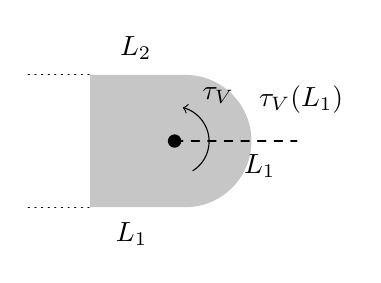
\begin{tikzpicture}[line cap=round,line join=round,scale=1.05]
  \path[fill=gray!45] (0,0) -- (0,1.6) -- (1.15,1.6)
    arc[start angle=90,end angle=-90,radius=0.8] -- cycle;
  \draw[dotted] (-0.75,1.6) -- (0,1.6);
  \draw[dotted] (-0.75,0) -- (0,0);
  \fill (1.02,0.8) circle (2.3pt);
  \draw[dashed] (1.02,0.8) -- (2.5,0.8);
  \draw[->] (1.24,0.44) arc[start angle=-58,end angle=76,radius=0.42];
  \node at (1.55,1.35) {$\tau_V$};
  \node at (0.55,1.92) {$L_2$};
  \node at (0.5,-0.32) {$L_1$};
  \node at (2.55,1.3) {$\tau_V(L_1)$};
  \node at (2.05,0.5) {$L_1$};
\end{tikzpicture}
\caption{}\label{fig:monodromy-cut-open}
\end{figure}
于是，\eqref{eq:floer-cocycle-c} 就是相伴的\trInvariant{}$C\Phi_{E^c/S^c}$，其中所用的是一个（\trRegular{}的）\trRelative\trPerturbationDatum，它与已定的\trFloerDatum{}选取\trCompatible。
第二份数据将是 $\mu^2(c,\cdot)$ 与零映射之间的一个\trChainHomotopy，即
\begin{equation}\label{eq:chain-homotopy-k}
\boxed{\begin{gathered}
k\colon CF^{\mathrm{pr}}(L_0,L_1)\longrightarrow CF^{\mathrm{pr}}(L_0,L_2),\\
\mu^1(k(\cdot))+k(\mu^1(\cdot))+\mu^2(c,\cdot)=0.
\end{gathered}}
\end{equation}
正如所期望的，这是由一个带\trStriplikeEnd{}的\trLefschetzFibration{}\trFamily{}构造出来的，该\trFamily{}依赖于一个参数 $r\in[0;1]$。在这一端，即 $r=0$ 处，取三\trPointedDisc{}上的平凡\trFibration，带\trLagrange\trBoundaryCondition{}$(L_0,L_1,L_2)$。配上一个适当的\trPerturbationDatum{}后，与之相伴的\trInvariant{}恰好给出 $\mu^2$ 本身。现在取出向两端中的一个，即\trLabel{}为 $(L_1,L_2)$ 的那个，把它\trGluing{}到 $E^c\to S^c$ 的入向端上。这一步应当以较大的\trGluingLength{}来进行，使得\trPseudoholomorphic\trSection{}的零维\trModuliSpace{}的\trGluing{}公式在上链层面上成立。所得结果记作 $E^{k,0}\to S^{k,0}$，是一个配有移动\trBoundaryCondition{}$F^{k,0}$ 与\trRelative\trPerturbationDatum{}的\trFibration，其相伴的\trInvariant{}恰为 $\mu^2(c,\cdot)$。它的两幅图像显示于\cref{fig:chain-homotopy-families}，二者仅在我们心目中剖开基的方式上有所不同。在另一端点 $r=1$ 处，我们按如下方式进行。
\begin{figure}[htbp]
\centering
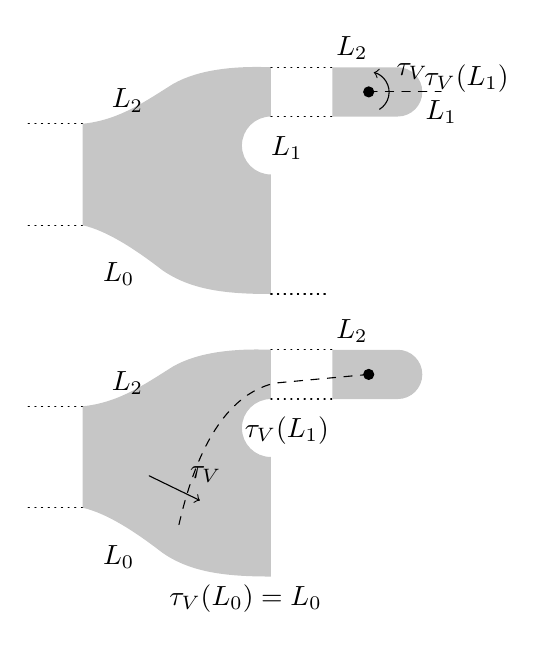
\begin{tikzpicture}[line cap=round,line join=round,scale=0.92]
\begin{scope}
  \path[fill=gray!45] (0,0)
    .. controls (0.35,-0.08) and (0.75,-0.35) .. (1.1,-0.62)
    .. controls (1.5,-0.9) and (2.0,-0.95) .. (2.6,-0.95)
    -- (2.6,0.7) arc[start angle=270,end angle=90,radius=0.4] -- (2.6,2.18)
    .. controls (2.1,2.2) and (1.6,2.15) .. (1.25,1.95)
    .. controls (0.85,1.7) and (0.5,1.45) .. (0,1.4) -- cycle;
  \draw[dotted] (-0.75,1.4) -- (0,1.4);
  \draw[dotted] (-0.75,0) -- (0,0);
  \draw[dotted] (2.6,2.18) -- (3.45,2.18);
  \draw[dotted] (2.6,1.5) -- (3.45,1.5);
  \path[fill=gray!45] (3.45,1.5) -- (3.45,2.18) -- (4.35,2.18)
    arc[start angle=90,end angle=-90,radius=0.34] -- cycle;
  \fill (3.95,1.84) circle (2.2pt);
  \draw[dashed] (3.95,1.84) -- (4.95,1.84);
  \draw[->] (4.1,1.6) arc[start angle=-58,end angle=76,radius=0.28];
  \node at (4.55,2.12) {$\tau_V$};
  \node at (0.62,1.72) {$L_2$};
  \node at (0.5,-0.68) {$L_0$};
  \node at (2.82,1.06) {$L_1$};
  \node at (3.72,2.44) {$L_2$};
  \node at (5.3,2.02) {$\tau_V(L_1)$};
  \node at (4.95,1.56) {$L_1$};
\end{scope}
  \draw[dotted] (2.6,-0.95) -- (3.35,-0.95);
\begin{scope}[shift={(0,-3.9)}]
  \path[fill=gray!45] (0,0)
    .. controls (0.35,-0.08) and (0.75,-0.35) .. (1.1,-0.62)
    .. controls (1.5,-0.9) and (2.0,-0.95) .. (2.6,-0.95)
    -- (2.6,0.7) arc[start angle=270,end angle=90,radius=0.4] -- (2.6,2.18)
    .. controls (2.1,2.2) and (1.6,2.15) .. (1.25,1.95)
    .. controls (0.85,1.7) and (0.5,1.45) .. (0,1.4) -- cycle;
  \draw[dotted] (-0.75,1.4) -- (0,1.4);
  \draw[dotted] (-0.75,0) -- (0,0);
  \draw[dotted] (2.6,2.18) -- (3.45,2.18);
  \draw[dotted] (2.6,1.5) -- (3.45,1.5);
  \path[fill=gray!45] (3.45,1.5) -- (3.45,2.18) -- (4.35,2.18)
    arc[start angle=90,end angle=-90,radius=0.34] -- cycle;
  \fill (3.95,1.84) circle (2.2pt);
  \draw[dashed] (3.95,1.84) -- (2.65,1.72)
    .. controls (1.95,1.55) and (1.55,0.75) .. (1.32,-0.28);
  \draw[->] (0.92,0.44) -- (1.62,0.1);
  \node at (1.7,0.46) {$\tau_V$};
  \node at (0.62,1.72) {$L_2$};
  \node at (0.5,-0.68) {$L_0$};
  \node at (2.82,1.06) {$\tau_V(L_1)$};
  \node at (3.72,2.44) {$L_2$};
  \node at (2.25,-1.25) {$\tau_V(L_0)=L_0$};
\end{scope}
  \draw[dotted] (2.6,-0.95) -- (3.35,-0.95);
\end{tikzpicture}
\caption{}\label{fig:chain-homotopy-families}
\end{figure}
取 $Z$ 上的平凡\trFibration。为其配备一个移动\trLagrange\trBoundaryCondition：它在 $\RR\times\{0\}$ 之上等于 $L_0$，而在 $\RR\times\{1\}$ 之上实现从 $L_2$ 到 $\tau_V(L_1)$ 的\trIsotopy。这意味着与两端相关联的\trLagrange\trSubmanifold{}对分别是 $(L_0,L_2)$ 与 $(L_0,\tau_V(L_1))$。对后一对，我们取的\trFloerDatum{}是 $(L_0,L_1)$ 的\trFloerDatum{}在 $\tau_V$ 下的像，这里要注意 $\tau_V(L_0)=\tau_V(V)=V=L_0$。我们还要标记一个边界点 $z^+\in\RR\times\{0\}$。现在取我们原来的 $\pi\colon E\to S$，为其配备一个标准\trBoundaryCondition{}$F$：它在 $\ast$ 之上的\trFiber{}中应等于 $L_0$，并且在该点附近应是\trLocallyConstant{}的。最后，沿 $z^+$ 与 $z^-=\ast$ 作\trBoundaryConnectedSum，把这两个\trFibration{}\trGluing{}在一起，并将所得结果记作 $E^{k,1}\to S^{k,1}$；见\cref{fig:boundary-sum-k1}。这是\cref{thm:fibre-product-vanishing}中所讨论的那个过程的一个实例，而且事实上\cref{thm:cochain-level-vanishing}在此适用；于是，只要把\trGluingParameter{}选得适当小，就能保证 $E^{k,1}$ 的\trPseudoholomorphic\trSection{}的一切零维\trModuliSpace{}或者为空（$n>1$），或者由偶数个点组成（$n=1$）。
\begin{figure}[htbp]
\centering
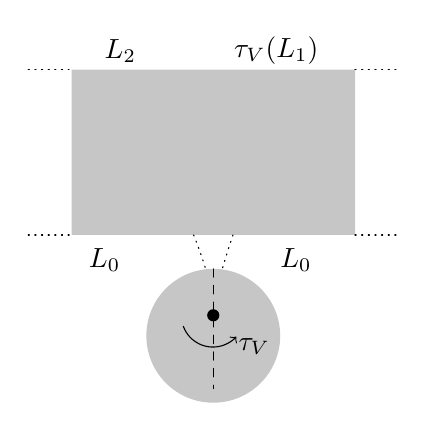
\begin{tikzpicture}[line cap=round,line join=round,scale=1.0]
  \path[fill=gray!45] (0,0) -- (1.55,0) -- (2.05,0) -- (3.6,0)
    -- (3.6,2.1) -- (0,2.1) -- cycle;
  \draw[dotted] (-0.55,2.1) -- (0,2.1);
  \draw[dotted] (3.6,2.1) -- (4.15,2.1);
  \draw[dotted] (-0.55,0) -- (0,0);
  \draw[dotted] (3.6,0) -- (4.15,0);
  \draw[dotted] (1.55,0) .. controls (1.68,-0.32) and (1.72,-0.5) .. (1.78,-0.68);
  \draw[dotted] (2.05,0) .. controls (1.94,-0.32) and (1.9,-0.5) .. (1.84,-0.68);
  \path[fill=gray!45] (1.8,-1.28) circle (0.85);
  \fill (1.8,-1.02) circle (2.2pt);
  \draw[dashed] (1.8,-0.43) -- (1.8,-1.95);
  \draw[->] (1.42,-1.16) arc[start angle=200,end angle=318,radius=0.4];
  \node at (2.32,-1.42) {$\tau_V$};
  \node at (0.62,2.34) {$L_2$};
  \node at (2.6,2.34) {$\tau_V(L_1)$};
  \node at (0.42,-0.32) {$L_0$};
  \node at (2.85,-0.32) {$L_0$};
\end{tikzpicture}
\caption{}\label{fig:boundary-sum-k1}
\end{figure}
把\cref{fig:chain-homotopy-families}与\cref{fig:boundary-sum-k1}直接对照即可看出：的确存在由\trFibration{}$E^{k,r}\to S^{k,r}$ 与\trBoundaryCondition{}$F^{k,r}$ 组成的一个单参数\trFamily，它把我们已对 $r\in\{0,1\}$ 构造出的那两个衔接起来。这些\trFibration{}在无穷远处（即在诸\trStriplikeEnd{}之上）的结构对一切 $r$ 都相同。选取\trRelative\trPerturbationDatum{}的一个\trFamily，使其在 $r=0,1$ 时与先前构造的相一致，并考察由此得到的\trParametrization{}的\trPseudoholomorphic\trSection{}\trModuliSpace。通过对这些空间中的\trIsolated{}点作计数，便定义出一个\trHomomorphism{}$k\colon CF^{\mathrm{pr}}(L_0,L_1)\cong CF^{\mathrm{pr}}(L_0,\tau_V(L_1))\to CF^{\mathrm{pr}}(L_0,L_2)$，它是 $C\Phi_{E^{k,0}/S^{k,0}}$ 与 $C\Phi_{E^{k,1}/S^{k,1}}$ 之间的一个\trChainHomotopy，从而恰好具有想要的性质 \eqref{eq:chain-homotopy-k}。
在构造 $c$ 的过程中，某些选取是不得不作的，因为无论\trBoundaryCondition{}还是\trPerturbationDatum{}都不完全是\trCanonical{}的。即便已经指定了这些，在定义\trFamily{}$E^{k,r}\to S^{k,r}$ 时仍有一些别的选取，而这些选取又会反过来影响 $k$。不过，在这两种情形中，参数空间都是道路\trConnected{}的，因此可以在任何两种可能性之间\trSmooth{}地移动。具体地说，这意味着：若 $(c,k)$ 与 $(\tilde c,\tilde k)$ 是用两个不同的选取定义的，则可以考虑多带一个参数的\trModuliSpace，从而找到
\begin{equation}\label{eq:cocycle-homotopy-independence}
\boxed{\begin{gathered}
\gamma\in CF^{\mathrm{pr}}(L_1,L_2),\\
\kappa\colon CF^{\mathrm{pr}}(L_0,L_1)\longrightarrow CF^{\mathrm{pr}}(L_0,L_2),\\
\mu^1(\gamma)+c+\tilde{c}=0,\\
\mu^1(\kappa(\cdot))+\kappa(\mu^1(\cdot))+\mu^2(\gamma,\cdot)+k+\tilde{k}=0.
\end{gathered}}
\end{equation}
这不过是我们先前那些考虑的一个直截了当的推广，因此我们不再解释其细节。作为替代，我们现在要依据 §5 的代数理论来解读这一结果。
\begin{remark}\label{thm:gradings-signs-provisional}
注意，我们的\trFloer{}理论框架至今尚未具备\trGrading，而且我们是在 $\mathrm{char}(\KK)=2$ 中工作的，那里符号是平凡的（上面诸公式中这两者的缺席都显而易见）。不过，\cref{thm:ungraded-category-remark}在此同样适用：首先，为\trUngraded{}的\trACategory{}重做一遍代数理论是相当容易的；其次，目前这个语境只是暂时性的，往后会被修改以纳入恰当的\trGrading{}与符号。记住这一点，我们便可以毫无顾忌地援引 §5 的结果了。
\end{remark}
具体地说，\cref{thm:quasi-representative-criterion}(i) 连同 \eqref{eq:floer-cocycle-c} 与 \eqref{eq:chain-homotopy-k} 表明，$(c,k)$ 给出\trAinfty-模的\trCohomology\trCategory{}中的一个\trMorphism{}$\scr{T}_{Y_0}(\scr{Y}_1)\to\scr{Y}_2$。类似地，\cref{thm:quasi-representative-criterion}(ii) 与 \eqref{eq:cocycle-homotopy-independence} 表明这个\trMorphism{}是\trCanonical{}的；也就是说，它不依赖于在定义用来给出 $c$ 与 $k$ 的\trLefschetzFibration{}和\trModuliSpace{}时所作的那些辅助选取。
